\documentclass[11pt,a4paper]{article}
\usepackage[margin=2.4cm]{geometry}
\usepackage{amsmath,amssymb}
\usepackage{graphicx}
\usepackage{booktabs}
\usepackage{listings}
\usepackage{xcolor}
\usepackage[colorlinks=true,linkcolor=blue!50!black,citecolor=blue!50!black,urlcolor=blue!50!black]{hyperref}
\usepackage{natbib}
\usepackage{caption}
\captionsetup{font=small,labelfont=bf}
\lstset{basicstyle=\ttfamily\scriptsize,columns=fullflexible,breaklines=true,
        frame=single,rulecolor=\color{gray!50},keywordstyle=\color{blue!60!black},
        commentstyle=\color{green!40!black},language=Python,showstringspaces=false}
\newcommand{\dd}{\mathrm{d}}
\newcommand{\rc}{r_c}
\newcommand{\Rb}{R_b}
\newcommand{\Rmax}{R_{\max}}

\title{The disc\\[4pt]
\large The disc that the seed's own angular momentum would make, and how\\
the gas settles into it\\[2pt]
\normalsize A companion note to \emph{From a primordial fluctuation to an idealised rotation curve}, Sect.~6.5}
\author{B. R. Parodi}
\date{23 October 2026; extended 29 October 2026}

\begin{document}
\maketitle

\begin{abstract}
\noindent \emph{Part~I.} In the seed of the main paper every shell rotates rigidly
with the specific angular momentum it receives by turnaround, $j\propto M$. If the
gas of each mass element keeps its own angular momentum and settles on a circular
orbit in the final rotation curve, the disc that forms is fixed completely by the
seed. We derive its surface density in closed form for a flat rotation curve,
compute it numerically for the P18 curve with its core, and compare it with an
exponential disc and with the relation of \citet{Mo1998} used in the main paper. The
seed disc is close to exponential between one and four scale lengths, but it has
twice the exponential mass inside half a scale length and a sharp edge at
$\Rmax=3\sqrt2\lambda GM/v\simeq4.3\,R_d$. Its scale length is 1.06 to 1.4 times the
Mo--Mao--White value, and it depends only weakly on the spin. This lowers the
inferred retained fraction of angular momentum $f_j$ and leaves the failed spin test
as it is. \emph{Part~II.} How does a gas parcel arriving on a tilted orbit join the
disc? A free particle cannot: its orbit keeps its plane, and with its angular
momentum conserved it cannot spiral in. We set up the simplest model with
dissipation and a preferred axis: a drag towards gas that rotates about $z$, at a
rate $\kappa$ times the orbital frequency, with the flow rotating at a fraction $f$
of the circular speed. Where the curve is flat, the parcel spirals in on an exact
logarithmic spiral ($\sin p=\kappa$ for $f=0$); for weak drag
$\tan p=\kappa(1-f)/(1+\dd\ln v_c/\dd\ln R)$, so the pitch halves in the core of
P18. The tilt decays as $\tan(i/2)\propto r^{f/[2(1-f)]}$: without a rotating flow the
orbit never settles into the disc. On the sphere of directions the path is an
inclined great circle whose tilt decays, not a loxodrome; the loxodrome survives in
geometry, since its stereographic projection is an exact logarithmic spiral. The
model describes the paths of gas parcels, not spiral arms.
\end{abstract}

\tableofcontents
\bigskip

\part{The disc of the seed}

\section{Motivation}

The main paper tests the energy closure with discs: if the stellar disc
keeps a fraction $f_j$ of the seed's specific angular momentum, then
$R_d/\rc=f_j\lambda y/\sqrt2$ (its Sect.~6.5). This relation assumes an
exponential disc in a flat rotation curve, for which the specific angular
momentum is $j_d=2vR_d$ \citep{Fall1980,Mo1998}. But the seed carries
more information than its mean angular momentum: it fixes how the
angular momentum is \emph{distributed} over its mass. Under detailed
conservation, each mass element keeping its own $j$
\citep{Mestel1963,Fall1980}, this distribution fixes the disc. The
question of Part~I is whether the disc so obtained is exponential, and
how its scale length compares with the Mo--Mao--White value. Part~II asks how
a gas parcel arriving on a tilted orbit joins this disc.

\section{Theory}

\subsection{Angular momentum of the seed}

As in the main paper we use units with $G=v=1$, where $v$ is the flat
speed, and measure masses in units of the seed mass $M_{\rm tot}$. A shell
enclosing the mass $M$ turns around at $R_{\rm ta}=2GM/v^2$ and receives
by then, through tidal torques, the specific angular momentum
\begin{equation}
  j_{\rm sh}(M)=\sqrt2\,\lambda\,vR_{\rm ta}=2\sqrt2\,\lambda\,\frac{GM}{v},
  \label{eq:jsh}
\end{equation}
chosen so that the total angular momentum, $J=\int_0^Mj_{\rm sh}\,\dd M'=\sqrt2\lambda GM^2/v$,
returns the spin parameter of \citet{Peebles1969},
$\lambda=J|E|^{1/2}/(GM^{5/2})$ with $|E|=\tfrac12v^2M$, for every $M$.
Each shell rotates rigidly about a common axis $z$. A mass element at
polar angle $\theta$ has $j_z=\omega R^2\sin^2\theta$, and averaging
$\sin^2\theta$ over the sphere ($\langle\sin^2\theta\rangle=\tfrac23$)
gives $j_{\rm sh}=\tfrac23\omega R^2$; hence
\begin{equation}
  j_z=\tfrac32\,j_{\rm sh}(M)\,\sin^2\theta
     =3\sqrt2\,\lambda\,\frac{GM}{v}\,(1-\mu^2),\qquad \mu=\cos\theta .
  \label{eq:jz}
\end{equation}
Since the shells are equally spaced in $M$ and the mass of a shell is
spread uniformly in $\mu$, the seed is a population of mass elements
with $M/M_{\rm tot}$ and $\mu$ uniformly distributed in $[0,1]$. The
largest angular momentum, on the equator of the outermost shell, is
$j_{\max}=3\sqrt2\lambda GM_{\rm tot}/v$, and the mean is
$\langle j_z\rangle=j_{\max}\langle M/M_{\rm tot}\rangle\langle1-\mu^2\rangle
=j_{\max}\cdot\tfrac12\cdot\tfrac23=\sqrt2\lambda GM_{\rm tot}/v$, the
specific angular momentum of the seed.

\subsection{Detailed conservation and the disc}

Let a fraction of the matter be gas that keeps a fraction $f_j$ of its
own $j_z$ and settles on the circular orbit with that angular momentum in
the final rotation curve $v_c(R)$:
\begin{equation}
  R\,v_c(R)=f_j\,j_z .
  \label{eq:orbit}
\end{equation}
Then the distribution of $j_z$ over the mass becomes the distribution of
disc mass over radius. We take the gas to be a fixed fraction of every
mass element, so the disc mass $M_d$ is distributed as the seed's
$j_z$.

\paragraph{Flat rotation curve (analytic).} With $v_c=v$ the orbit
radius is $R=f_jj_z/v$, and with $S=R/\Rmax$,
\begin{equation}
  \Rmax=\frac{f_jj_{\max}}{v}=3\sqrt2\,f_j\lambda\,\frac{GM_{\rm tot}}{v^2},
  \qquad S=\frac{M}{M_{\rm tot}}\,(1-\mu^2).
\end{equation}
The disc mass inside $S$ is the fraction of the unit square
$(M/M_{\rm tot},\mu)$ where $(M/M_{\rm tot})(1-\mu^2)<S$. For
$1-\mu^2<S$, i.e.\ $\mu>\sqrt{1-S}$, every $M$ qualifies; otherwise only
$M/M_{\rm tot}<S/(1-\mu^2)$. Hence
\begin{equation}
  F(S)\equiv\frac{M_d(<R)}{M_d}
  =\bigl(1-\sqrt{1-S}\bigr)+\int_0^{\sqrt{1-S}}\frac{S\,\dd\mu}{1-\mu^2}
  =1-\sqrt{1-S}+S\,\operatorname{artanh}\sqrt{1-S},
  \label{eq:F}
\end{equation}
using $\int\dd\mu/(1-\mu^2)=\operatorname{artanh}\mu$. Differentiating,
the two terms $\pm1/(2\sqrt{1-S})$ cancel and
$F'(S)=\operatorname{artanh}\sqrt{1-S}$, so the surface density,
$\Sigma=(\dd M_d/\dd R)/(2\pi R)$, is
\begin{equation}
  \Sigma(R)=\frac{M_d}{2\pi\Rmax^2}\,
  \frac{\operatorname{artanh}\sqrt{1-S}}{S},\qquad S=\frac{R}{\Rmax}\le1 .
  \label{eq:Sigma}
\end{equation}
Two limits show its character. Near the centre,
$\operatorname{artanh}\sqrt{1-S}\simeq\tfrac12\ln(4/S)$, so
$\Sigma\propto\ln(4/S)/S$: a central cusp, steeper than any exponential.
At the edge, $\operatorname{artanh}\sqrt{1-S}\simeq\sqrt{1-S}$, so
$\Sigma\to0$ as $\sqrt{1-S}$: the disc ends sharply at $\Rmax$, the
orbit of the equator of the outermost shell. In between,
Eq.~\eqref{eq:Sigma} is close to exponential (Fig.~\ref{fig:disc}a).

\paragraph{P18 rotation curve (numerical).} Inside the core the curve
rises, $v_c\simeq(2/\sqrt3)(v/\rc)R$, so Eq.~\eqref{eq:orbit} gives
$R\propto j_z^{1/2}$ instead of $R\propto j_z$: low-$j$ material lands
further out than in a flat curve, and the central cusp of
Eq.~\eqref{eq:Sigma} is softened. We invert Eq.~\eqref{eq:orbit} on a
grid for the P18 curve $v_c=v\sqrt{m(x)/x}$, $x=R/\rc$, with
$\rc=\Rb/y$ and the core ratio $y$ of the main paper (its core equation, Sect.~4.3, with
$\Lambda=0$; $y=50.5$ for $\lambda=0.035$), and sample $2\times10^6$ mass
elements from the uniform distribution of $(M/M_{\rm tot},\mu)$.

\paragraph{Scale length of a non-exponential disc.} For the comparison
with an exponential disc a scale length must be defined. We use two
definitions: an exponential fit to $\Sigma$ between one and four scale
lengths (iterated), as photometry would measure it, and the half-mass
radius divided by 1.678, its value for an exponential disc. The relation
of \citet{Mo1998} for a flat curve gives
$R_d^{\rm MMW}=f_j\langle j_z\rangle/(2v)=f_j\lambda GM_{\rm tot}/(\sqrt2v^2)$,
i.e.\ $R_d/\rc=f_j\lambda y/\sqrt2$ with $GM_{\rm tot}/v^2\simeq\Rb$.

\section{The code}

The script \texttt{seed\_disc.py} (Appendix~\ref{app:code}) does the
following. (i) It solves the core equation of the main paper for $y$.
(ii) It draws mass elements with uniform $M/M_{\rm tot}$ and $\mu$,
assigns $j_z$ from Eq.~\eqref{eq:jz}, and places each on the circular
orbit of Eq.~\eqref{eq:orbit} in the P18 curve, by interpolating the
monotonic function $Rv_c(R)$. (iii) It computes $\Sigma$, the enclosed
mass and the two scale lengths, and compares them with the analytic
flat-curve result, Eqs.~\eqref{eq:F} and \eqref{eq:Sigma}, and with an
exponential disc. (iv) It repeats the calculation for spins from 0.015
to 0.1 and makes Fig.~\ref{fig:disc}. Near the centre the closed form of
$m(x)$ loses precision through cancellation; the code uses the series
$m\simeq\tfrac43x^3$ for $x<10^{-3}$. It runs in about twenty seconds.

\section{Results}

\begin{figure}[t]
\centering
\includegraphics[width=\textwidth]{fig_seed_disc.png}
\caption{The disc made by the seed's own angular momentum ($f_j=1$,
$\Lambda=0$). (a) Surface density for $\lambda=0.035$: Monte Carlo in
the P18 curve (points), the analytic flat-curve result,
Eq.~\eqref{eq:Sigma} (solid), and an exponential disc with the same
scale length (dashed); dotted lines mark the core radius and the edge
$\Rmax$. (b) Enclosed disc mass, seed against exponential. (c) Ratio of
disc scale length to core radius against spin: seed disc with $R_d$ from
an exponential fit at 1--4 $R_d$ (filled) and from the half-mass radius
(open), and the relation of \citet{Mo1998} used in the main paper
(dashed). Green: the median and $1\sigma$ spread of the 79 SPARC dwarfs;
the observed values require $f_j<1$.}
\label{fig:disc}
\end{figure}

For the median spin, $\lambda=0.035$ ($y=50.5$, $\rc=0.020\,\Rb$), the
script gives the following.
\begin{itemize}
\item \emph{Shape.} Between one and four scale lengths the disc is close
  to exponential (Fig.~\ref{fig:disc}a). Inside $0.5\,R_d$ it holds 19\%
  of its mass, twice the 9\% of an exponential disc; the half-mass radius
  is $1.27\,R_d$ instead of $1.68\,R_d$ (Fig.~\ref{fig:disc}b). The disc
  ends at $\Rmax=0.149\,\Rb=4.3\,R_d$.
\item \emph{Effect of the core.} The rising inner curve moves low-$j$
  material outward: inside $S=0.1$ the P18 curve places 15\% of the disc
  mass, the flat curve 23\%. Beyond $S\simeq0.3$ the two agree.
\item \emph{Scale length.} The exponential fit gives
  $R_d=0.035\,\Rb$, $R_d/\rc=1.76f_j$, 1.40 times the Mo--Mao--White
  value $1.26f_j$; the half-mass definition gives $1.33f_j$, 1.06 times
  that value. The difference between the two definitions measures how far
  the seed disc is from exponential.
\item \emph{Dependence on spin.} $R_d/\rc$ changes little with $\lambda$
  (Fig.~\ref{fig:disc}c): $\dd\ln(R_d/\rc)/\dd\ln\lambda=0.16$ at
  $\lambda=0.035$, with a broad maximum near $\lambda\simeq0.05$. The
  reason is the same as in the main paper: a larger spin makes the disc
  larger but also the core larger ($y$ smaller), and the two nearly
  cancel.
\end{itemize}

\section{Relevance to the main paper}

\paragraph{The retained fraction $f_j$.} The observed median
$R_d/\rc=0.67$ is reproduced with a smaller $f_j$ than with the
Mo--Mao--White relation: smaller by the factor 1.06 to 1.4, so the
$f_j\simeq0.77$ of the main paper becomes 0.55--0.73. This is within the
range usually inferred for discs and does not change any conclusion.

\paragraph{The spin test.} The test of the main paper rests on the
\emph{width} of the distribution of $R_d/\rc$. A constant factor does not
change the width, and the weak dependence on $\lambda$ found here (0.16)
is the same as with the Mo--Mao--White relation. The predicted
distribution therefore stays as narrow as before, and the spin test
fails as before.

\paragraph{The shape of real discs.} Detailed conservation of the seed's
angular momentum gives too much mass at the centre and a sharp edge,
the well-known angular-momentum distribution problem of discs that form
by detailed conservation \citep{Dalcanton1997,Bullock2001,vandenBosch2001}.
Late-type dwarfs are bulgeless, so the central excess must have been
removed or redistributed; preferential removal of low-angular-momentum
gas by feedback is the usual explanation
\citep{Governato2010,Brook2011}. The edge near $4.3\,R_d$ is reminiscent
of the truncations and breaks observed in disc profiles at three to five
scale lengths \citep{vanderKruit1979,Pohlen2006}, but a dissipational
disc need not keep the sharp edge of Eq.~\eqref{eq:Sigma}.


\part{How the gas settles into the disc}

\section{From the loxodrome picture to a model}

The idea to be modelled is this: matter collapsing in a rotating protogalaxy winds
around a shrinking sphere along a spiral, and when the system flattens, the spiral
becomes a logarithmic spiral in the disc. Two simple facts show what a model must
contain.

\emph{A free particle does not wind around a sphere.} In a spherical potential the
force is radial, so the torque $\mathbf r\times\mathbf F$ vanishes and the angular
momentum \emph{vector} $\mathbf L$ is conserved. The particle moves in the fixed plane
perpendicular to $\mathbf L$, and its direction $\hat{\mathbf r}$ moves on a great
circle of the sphere of directions, never on a loxodrome or any other spiral.

\emph{A free particle does not spiral in steadily.} With $j=r v_\varphi$ conserved,
the azimuthal speed grows as $1/r$ when $r$ shrinks, and the particle bounces back
from its centrifugal barrier. Even if one imposes a steady inflow, $\dot r=-kr$, the
conserved $j$ gives $\dot\varphi=j/r^2$ and hence $\dd r/\dd\varphi=-(k/j)r^3$, i.e.\
$r\propto\varphi^{-1/2}$: a lituus, not a logarithmic spiral.

Both facts point to the same missing ingredient: \emph{dissipation}. (Part~I
assumed it: there each gas element simply settles on the circular orbit of its own
angular momentum.) Gas can lose
angular momentum and energy in collisions between streams, in shocks and through
viscosity; dark matter cannot. The model is therefore a model for the gas of the
seed, which in the paper settles with its angular momentum into the disc
(Sect.~6.5). A second ingredient is needed to make the disc \emph{one} plane: a
preferred axis. In the model it is the rotation of the gas that has already
settled.

% ==========================================================================
\section{The geometry of constant angles}

\subsection{The logarithmic spiral}
In plane polar coordinates $(r,\varphi)$ a curve crosses the circle $r=$\,const at
the \emph{pitch angle} $p$ given by
\begin{equation}
  \tan p=-\frac{1}{r}\frac{\dd r}{\dd\varphi}=-\frac{v_r}{v_\varphi},
  \label{eq:pitch}
\end{equation}
where $v_r=\dot r$ and $v_\varphi=r\dot\varphi$ for a particle moving along the
curve. A constant pitch gives $\ln r=-\varphi\tan p+$\,const, the
\emph{logarithmic spiral} $r=r_0e^{-\varphi\tan p}$. Kinematically: \emph{a particle
moves on a logarithmic spiral if and only if the ratio of its radial to its
azimuthal velocity is constant.}

\subsection{The loxodrome}
On a sphere with latitude $\psi$ and longitude $\lambda$, a loxodrome crosses all
meridians at the same angle $\alpha$. A step along it has meridional length $\dd\psi$
and zonal length $\cos\psi\,\dd\lambda$ (on the unit sphere), so
\begin{equation}
  \tan\alpha=\frac{\cos\psi\,\dd\lambda}{\dd\psi}=\frac{v_\lambda}{v_\psi},
  \qquad
  \lambda-\lambda_0=\tan\alpha\;\ln\tan\Bigl(\frac\pi4+\frac\psi2\Bigr).
  \label{eq:lox}
\end{equation}
Again a constant ratio, now of the zonal to the meridional velocity. The quantity
$y=\ln\tan(\pi/4+\psi/2)$ is the ordinate of Mercator's map, on which loxodromes are
straight lines.

\subsection{Stereographic projection turns loxodromes into logarithmic spirals}
Project the unit sphere from its south pole onto the equatorial plane. A point at
latitude $\psi$ and longitude $\lambda$ lands at polar angle $\lambda$ and radius
\begin{equation}
  \rho=\frac{\cos\psi}{1+\sin\psi}=\tan\Bigl(\frac\pi4-\frac\psi2\Bigr)=e^{-y}.
\end{equation}
On a loxodrome $y=(\lambda-\lambda_0)\cot\alpha$, so its image is
\begin{equation}
  \rho=e^{-(\lambda-\lambda_0)\cot\alpha}:
\end{equation}
an exact logarithmic spiral, with pitch $p=90^\circ-\alpha$. The reason is that
stereographic projection is \emph{conformal}: it preserves angles. It maps meridians
onto radial lines, and a curve that crosses all meridians at the angle $\alpha$ is
mapped onto a curve that crosses all radial lines at the same angle
(Fig.~\ref{fig:lox}).

This is the precise sense in which ``a spiral on a sphere becomes a logarithmic
spiral in the plane''. It is a statement of geometry, however, not of dynamics.
Moreover, a loxodrome runs from pole to pole and never settles onto the equator;
a particle that is to end up in a disc must do something else. The rest of Part~II
asks what.

\begin{figure}[h]
\centering
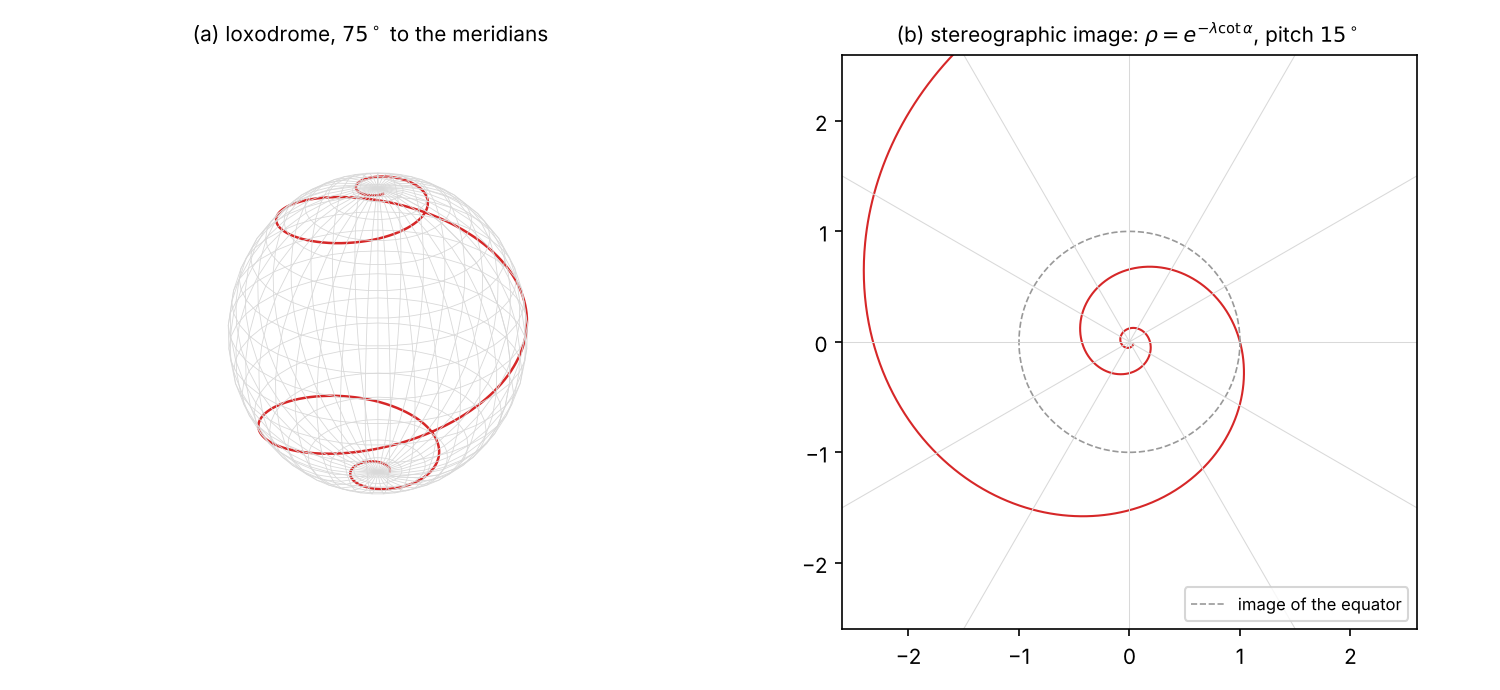
\includegraphics[width=0.92\textwidth]{fig_loxodrome.png}
\caption{(a)~A loxodrome crossing the meridians at $75^\circ$. (b)~Its stereographic
projection from the south pole: the logarithmic spiral
$\rho=e^{-\lambda\cot\alpha}$, with pitch $15^\circ$. Grey lines: images of
meridians (radial lines) and of the equator (unit circle). Script:
\texttt{code/spiral\_figs.py}.}
\label{fig:lox}
\end{figure}

% ==========================================================================
\section{The model}

A gas parcel moves in the potential $\Phi$ of the galaxy, here P18 with
$\dd\Phi/\dd r=GM(r)/r^2$, and feels a drag towards the local mean flow of the gas:
\begin{equation}
  \ddot{\mathbf r}=-\nabla\Phi-\gamma\bigl(\dot{\mathbf r}-\mathbf u\bigr),
  \qquad
  \mathbf u=f\,\Omega(r)\,\hat{\mathbf z}\times\mathbf r,
  \qquad
  \gamma=\kappa\,\Omega(r),
  \label{eq:model}
\end{equation}
with $\Omega=v_c/r$ the circular angular frequency. The flow $\mathbf u$ rotates about
the $z$-axis with angular speed $f\Omega$: in the equatorial plane at a fraction $f$
of the circular speed ($0\le f<1$; gas supported partly by pressure, or still
assembling, rotates more slowly than circular). The drag rate is a fixed fraction
$\kappa$ of the orbital frequency, so that it acts with the same strength per orbit
at every radius. In the flat part of the curve this makes the model
\emph{scale-free}: no length scale is introduced, which is why logarithmic spirals
appear.

The parcel's velocity has three components, radial $v_r$, meridional $v_\psi$
(towards or away from the poles) and azimuthal $v_\varphi$ (about $z$). The model
couples them as follows.
\begin{itemize}
\item The radial motion is pulled by gravity and damped by the drag.
\item The angular momentum changes by the torque of the drag,
  \begin{equation}
    \dot{\mathbf L}=-\gamma\,\mathbf L
    +\gamma f\Omega\,\bigl(r^2\hat{\mathbf z}-z\,\mathbf r\bigr),
    \label{eq:torque}
  \end{equation}
  where the first term shrinks $\mathbf L$ without turning it, and the second, from
  the rotating flow, adds angular momentum about $z$ and turns $\mathbf L$ towards
  $\hat{\mathbf z}$.
\end{itemize}
Equation~\eqref{eq:torque} contains the first result. \emph{Without a rotating flow,
$f=0$, the torque is parallel to $\mathbf L$: the orbit loses angular momentum and
spirals in, but in its own, tilted plane.} A drag towards rest cannot make a disc.
Only friction against matter that already rotates about an axis can bring orbits
into one plane.

% ==========================================================================
\section{Analytic results}

\subsection{The flat part: an exact logarithmic spiral}\label{sec:flat}
Where $v_c=v$, look for a steady inflow in the equatorial plane with constant
velocity ratios, $v_r=-Av$ and $v_\varphi=Bv$. Along such a path $v_r$ and
$v_\varphi$ do not change, and the equations of motion in polar coordinates,
\begin{equation}
  \dot v_r-\frac{v_\varphi^2}{r}=-\frac{v^2}{r}-\gamma v_r,
  \qquad
  \dot v_\varphi+\frac{v_rv_\varphi}{r}=-\gamma\,(v_\varphi-fv),
\end{equation}
with $\gamma=\kappa v/r$, reduce to two algebraic conditions:
\begin{equation}
  B^2=1-\kappa A,\qquad AB=\kappa\,(B-f).
\end{equation}
Eliminating $A$,
\begin{equation}
  B^3+(\kappa^2-1)\,B=\kappa^2f,\qquad
  \tan p=\frac AB=\frac{\kappa\,(B-f)}{B^2}.
  \label{eq:flat}
\end{equation}
Since the ratio $v_r/v_\varphi$ is constant, the path is an exact logarithmic spiral
(Eq.~\ref{eq:pitch}). For $f=0$, $A=\kappa$ and $B=\sqrt{1-\kappa^2}$, so that
\begin{equation}
  \sin p=\kappa\qquad(f=0).
\end{equation}
Two remarks. The parcel moves at slightly less than circular speed ($B<1$), since
the drag holds it back. And the inflow speed $Av$ is a constant fraction of $v$: the
parcel drifts inwards by the same factor per turn at every radius, which is the
defining property of a logarithmic spiral. Values are given in Table~\ref{tab:flat}.

\begin{table}[h]
\centering\small
\caption{Steady inflow in the flat part, Eq.~\eqref{eq:flat}, and pitch in the
solid-body core, Eq.~\eqref{eq:core}; $q$ is the decay rate of the tilt per radian,
Eq.~\eqref{eq:tilt}.}
\label{tab:flat}
\begin{tabular}{rrrrrrr}
\toprule
$\kappa$ & $f$ & $B$ & $A$ & pitch, flat part & $q$ & pitch, core\\
\midrule
0.1 & 0 & 0.995 & 0.100 & $5.7^\circ$ & 0 & $2.9^\circ$\\
0.1 & 0.5 & 0.998 & 0.050 & $2.9^\circ$ & 0.025 & $1.4^\circ$\\
0.2 & 0 & 0.980 & 0.200 & $11.5^\circ$ & 0 & $5.7^\circ$\\
0.2 & 0.5 & 0.990 & 0.099 & $5.7^\circ$ & 0.051 & $2.9^\circ$\\
0.3 & 0.5 & 0.978 & 0.147 & $8.5^\circ$ & 0.078 & $4.3^\circ$\\
0.5 & 0.5 & 0.940 & 0.234 & $14.0^\circ$ & 0.142 & $7.1^\circ$\\
0.5 & 0.8 & 0.977 & 0.091 & $5.3^\circ$ & 0.210 & $2.8^\circ$\\
\bottomrule
\end{tabular}
\end{table}

\subsection{Any rotation curve: the pitch follows the slope of the curve}
For weak drag, $\kappa\ll1$, the parcel stays close to a circular orbit, and its
inflow is set by its angular-momentum budget. On a near-circular orbit $j=rv_c(r)$,
so moving inwards by $\dd r$ costs
\begin{equation}
  \frac{\dd j}{\dd r}=v_c+r\frac{\dd v_c}{\dd r}=v_c\,(1+\beta_s),
  \qquad\beta_s\equiv\frac{\dd\ln v_c}{\dd\ln R},
\end{equation}
while the drag removes angular momentum at the rate
$\dot j=-\gamma(v_c-fv_c)\,r=-\kappa(1-f)\,v_c^2$. The inflow speed is
$v_r=\dot j/(\dd j/\dd r)=-\kappa(1-f)\,v_c/(1+\beta_s)$, and hence
\begin{equation}
  \boxed{\;\tan p=\frac{\kappa\,(1-f)}{1+\dd\ln v_c/\dd\ln R}\;}
  \label{eq:general}
\end{equation}
In the flat part, $\beta_s=0$, this is the small-$\kappa$ limit of
Eq.~\eqref{eq:flat}. In a solid-body core, $\beta_s=1$, it is half as large: there
each step inwards costs twice as much angular momentum, because $j=\Omega r^2$
falls as $r^2$. For P18, $\beta_s$ falls from 1 at the centre to 0.54 at $\rc$, 0.27
at $2\rc$ and 0 at the maximum of the curve, $5.5\,\rc$, so that the inflow paths
open up from the core outwards (Fig.~\ref{fig:model}e).

In the harmonic core itself the model is linear and can be solved exactly. With
$\zeta=x+iy$ in the equatorial plane and $\Omega=\omega=(2/\sqrt3)\,v/\rc$ constant,
Eq.~\eqref{eq:model} becomes
$\ddot\zeta=-\omega^2\zeta-\kappa\omega(\dot\zeta-if\omega\zeta)$, whose solutions
are $\zeta\propto e^{st}$ with
\begin{equation}
  s^2+\kappa\omega\,s+\omega^2(1-i\kappa f)=0,\qquad
  \tan p=-\frac{{\rm Re}\,s}{{\rm Im}\,s},
  \label{eq:core}
\end{equation}
again an exact logarithmic spiral, since $\zeta\propto e^{({\rm Re}\,s)t}e^{i({\rm
Im}\,s)t}$. To first order in $\kappa$, $s=i\omega-\tfrac12\kappa\omega(1-f)$, which
is Eq.~\eqref{eq:general} with $\beta_s=1$.

\subsection{Settling into the disc}
Now let the orbit be tilted by the angle $i$ against the equatorial plane. Average
the torque~\eqref{eq:torque} over one revolution on a circle of radius $r$ in the
tilted plane. With unit vectors $\mathbf e_1$ along the line of nodes and $\mathbf
e_2$ in the plane, $\hat{\mathbf z}\cdot\mathbf e_2=\sin i$, one has $z=r\sin
i\sin\phi'$ and $\langle z\mathbf r\rangle=\tfrac12r^2\sin i\,\mathbf e_2$, where
$\phi'$ is the angle in the orbital plane. The part of the averaged torque
perpendicular to $\mathbf L$ is therefore $\tfrac12\gamma f\Omega r^2\sin i\;\mathbf
e_2$, which turns $\mathbf L$ towards $\hat{\mathbf z}$ at the rate
$\dd i/\dd t=-\gamma f\Omega r^2\sin i/(2j)$. With $j=Bvr$ and the orbital rate
$\dd\phi'/\dd t=Bv/r$,
\begin{equation}
  \frac{\dd i}{\dd\varphi}=-q\sin i,\qquad q=\frac{\kappa f}{2B^2},
  \qquad\text{so}\qquad
  \tan\frac i2=\tan\frac{i_0}2\;e^{-q\varphi}.
  \label{eq:tilt}
\end{equation}
The tilt decays exponentially with the angle turned, but only if $f>0$. Dividing by
the inflow per radian, $\dd\ln r/\dd\varphi=-\tan p$, gives the tilt as a function of
radius,
\begin{equation}
  \tan\frac i2\propto r^{\,q/\tan p}=r^{\,f/[2(B-f)]}\simeq r^{\,f/[2(1-f)]},
  \label{eq:tiltr}
\end{equation}
independent of $\kappa$. For $f=0.5$ the tilt falls as $r^{1/2}$: the parcel must
move in by a factor of four to halve its tilt. For $f=0.9$ it falls as $r^{4.5}$:
a flow that nearly co-rotates flattens the orbit long before the parcel has moved
far in. The thinness of a disc thus measures how close to co-rotation the gas was when
it settled. (In the core the pitch halves, so the exponent of
Eq.~\ref{eq:tiltr} doubles.)

\subsection{The path on the sphere}
What does the parcel's direction $\hat{\mathbf r}$ do? On a tilted orbit the latitude
oscillates, $\sin\psi=\sin i\,\sin\phi'$, once per revolution between $-i$ and $+i$.
As $i$ decays, the oscillation shrinks, and the path of $\hat{\mathbf r}$ on the
sphere of directions is a great circle that tilts down onto the equator turn by turn
(Fig.~\ref{fig:model}c). Its heading against the meridians is not constant, as for a
loxodrome, but turns towards the east: the path winds onto the equator instead of
running to a pole. Combined with the shrinking radius, the parcel moves on a sequence
of ever smaller spheres along ever flatter great circles, and ends on the logarithmic
spiral of Sect.~\ref{sec:flat} in the plane. This is the dynamical version of the
picture we started from: a spiral on a sphere that becomes a logarithmic spiral in a
disc.

% ==========================================================================
\section{Numerical check}

The equations~\eqref{eq:model} were integrated for parcels starting at $r=60\,\rc$
on the steady inflow of the flat part, but in a plane tilted by $40^\circ$
(\texttt{code/spiral\_model.py}). Figure~\ref{fig:model} and Table~\ref{tab:num} show the
results.

\begin{table}[h]
\centering\small
\caption{Predicted and measured pitch angle (in the orbital plane, averaged over
all passages through the given radii) and tilt decay rate.}
\label{tab:num}
\begin{tabular}{rrrrrrrr}
\toprule
$\kappa$ & $f$ & \multicolumn{2}{c}{pitch at $8$--$12\,\rc$} &
\multicolumn{2}{c}{pitch at $0.2$--$0.5\,\rc$} & \multicolumn{2}{c}{$\dd\ln\tan(i/2)/\dd\varphi$}\\
 & & predicted & measured & predicted & measured & predicted & measured\\
\midrule
0.2 & 0.5 & $5.7^\circ$ & $6.1^\circ$ & $3.1^\circ$ & $3.1^\circ$ & $-0.051$ & $-0.050$\\
0.3 & 0.5 & $8.5^\circ$ & $9.1^\circ$ & $4.6^\circ$ & $4.7^\circ$ & $-0.078$ & $-0.081$\\
0.2 & 0 & $11.5^\circ$ & $11.7^\circ$ & $6.2^\circ$ & $6.3^\circ$ & 0 & 0\\
\bottomrule
\end{tabular}
\end{table}

The predictions hold to a few per cent. The pitch in the flat part is slightly
larger than predicted while the orbit is still tilted: a tilted orbit sees the
rotating flow at an angle, so the effective $f$ is smaller (roughly $f\cos i$), and
the inflow faster. Once the orbit has settled, the measured pitch follows
Eq.~\eqref{eq:general} through the transition from the flat part to the core. For
$f=0$ the tilt stays exactly at $40^\circ$, as Eq.~\eqref{eq:torque} requires.

\begin{figure}[t]
\centering
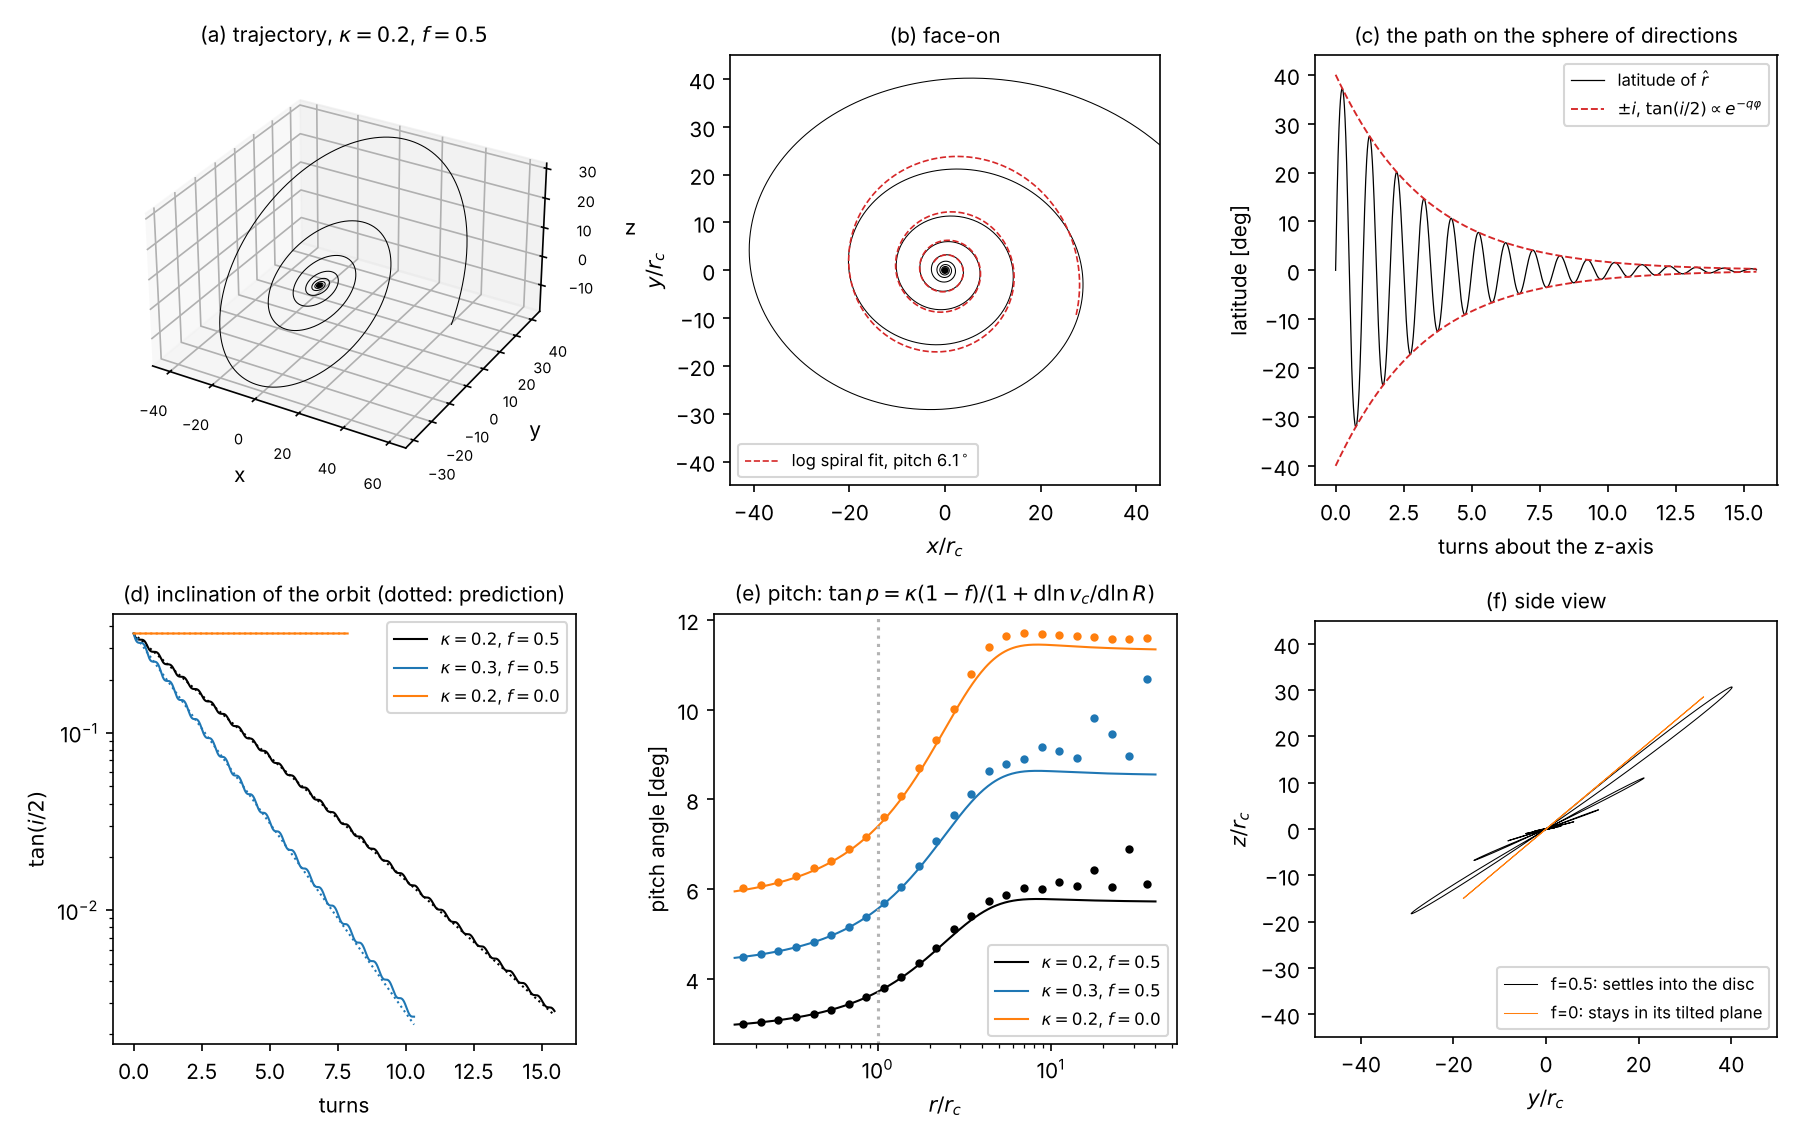
\includegraphics[width=\textwidth]{fig_spiral_model.png}
\caption{The model in the P18 potential (units $G=v=\rc=1$). (a)~Trajectory for
$\kappa=0.2$, $f=0.5$, starting at $60\,\rc$ in a plane tilted by $40^\circ$.
(b)~Face-on view with a logarithmic spiral fitted at $3$--$30\,\rc$ (pitch
$6.1^\circ$ in projection, against $5.7^\circ$ predicted for a settled orbit).
(c)~Latitude of the direction $\hat{\mathbf r}$ against the number of turns:
oscillations between $\pm i$, with the envelope of Eq.~\eqref{eq:tilt}. (d)~Tilt
of the orbit, $\tan(i/2)$, for three models; dotted: Eq.~\eqref{eq:tilt}.
(e)~Pitch angle against radius: points from the integrations, lines from
Eq.~\eqref{eq:general}. (f)~Side view along the line of nodes: with $f=0.5$ the
orbit settles into the disc; with $f=0$ it spirals in within its tilted plane.
Script: \texttt{code/spiral\_figs.py}.}
\label{fig:model}
\end{figure}

% ==========================================================================
\section{What the model means, and what it does not}
\begin{itemize}
\item \emph{It is a model for gas.} Dark matter has no drag; its orbits keep their
  planes and their angular momenta (companion note \emph{Halting and settling}). The model describes how a gas
  parcel of the seed, arriving on a tilted, nearly circular orbit after its shock at
  the front, would join the disc that the gas already in place has formed (paper,
  Sect.~6.5).
\item \emph{Logarithmic spirals come from scale freedom.} The paths are exactly
  logarithmic where the rotation curve is flat or rising linearly, because there the
  model has no length scale; in between, their pitch follows the slope of the curve,
  Eq.~\eqref{eq:general}. For P18 the pitch of the inflow halves from the flat part
  to the core.
\item \emph{A disc needs a rotating flow.} Without it ($f=0$) drag lets matter spiral
  in, but each parcel in its own plane. The rate of flattening per radius depends
  only on $f$, Eq.~\eqref{eq:tiltr}.
\item \emph{The paths are not spiral arms.} The arms of disc galaxies are patterns,
  density waves or transient swing-amplified features, through which the gas and
  stars move; material arms would wind up within a few rotations. The model's spirals
  are the paths of individual parcels, typically with pitch angles of a few degrees
  for $\kappa\lesssim0.3$, much tighter than typical arms (10--$30^\circ$). Their
  pitch also \emph{grows} with the shear of the rotation curve (larger in the flat
  part than in the core), while the arms of observed galaxies are reported to be
  \emph{tighter} where the shear is larger (Seigar et al.\ 2005, 2006); the two are
  different things.
\item \emph{The parameters are not derived.} $\kappa$ and $f$ summarise collisions,
  shocks and viscosity. A hydrodynamical simulation of the seed's gas would fix them;
  the model only shows what follows once they are given.
\end{itemize}

\begin{thebibliography}{99}
\bibitem[Binney \& Tremaine(2008)]{Binney2008} Binney, J., \& Tremaine, S. 2008, Galactic Dynamics, 2nd ed. (Princeton: Princeton University Press)
\bibitem[Brook et al.(2011)]{Brook2011} Brook, C.~B., Governato, F., Ro\v{s}kar, R., et al. 2011, MNRAS, 415, 1051
\bibitem[Bullock et al.(2001)]{Bullock2001} Bullock, J.~S., Dekel, A., Kolatt, T.~S., et al. 2001, ApJ, 555, 240
\bibitem[Dalcanton et al.(1997)]{Dalcanton1997} Dalcanton, J.~J., Spergel, D.~N., \& Summers, F.~J. 1997, ApJ, 482, 659
\bibitem[Fall \& Efstathiou(1980)]{Fall1980} Fall, S.~M., \& Efstathiou, G. 1980, MNRAS, 193, 189
\bibitem[Governato et al.(2010)]{Governato2010} Governato, F., Brook, C., Mayer, L., et al. 2010, Nature, 463, 203
\bibitem[Mestel(1963)]{Mestel1963} Mestel, L. 1963, MNRAS, 126, 553
\bibitem[Mo et al.(1998)]{Mo1998} Mo, H.~J., Mao, S., \& White, S.~D.~M. 1998, MNRAS, 295, 319
\bibitem[Peebles(1969)]{Peebles1969} Peebles, P.~J.~E. 1969, ApJ, 155, 393
\bibitem[Pohlen \& Trujillo(2006)]{Pohlen2006} Pohlen, M., \& Trujillo, I. 2006, A\&A, 454, 759
\bibitem[Seigar et al.(2005)]{Seigar2005} Seigar, M.~S., Block, D.~L., Puerari, I., Chorney, N.~E., \& James, P.~A. 2005, MNRAS, 359, 1065
\bibitem[Seigar et al.(2006)]{Seigar2006} Seigar, M.~S., Bullock, J.~S., Barth, A.~J., \& Ho, L.~C. 2006, ApJ, 645, 1012
\bibitem[van den Bosch et al.(2001)]{vandenBosch2001} van den Bosch, F.~C., Burkert, A., \& Swaters, R.~A. 2001, MNRAS, 326, 1205
\bibitem[van der Kruit(1979)]{vanderKruit1979} van der Kruit, P.~C. 1979, A\&AS, 38, 15
\end{thebibliography}

\appendix
\section{Code}\label{app:code}
Part~I: \texttt{code/seed\_disc.py} (listed below), output
\texttt{code/seed\_disc\_output.txt}. Part~II: \texttt{code/spiral\_model.py}
(analytic predictions and integrations; output \texttt{code/spiral\_model\_out.txt}),
\texttt{code/spiral\_figs.py} (the two figures of Part~II; it needs
\texttt{spiral\_runs.pkl}, written by \texttt{spiral\_model.py}) and
\texttt{code/p18core.py} (the P18 functions). Run the scripts from \texttt{code/}.
\lstinputlisting{code/seed_disc.py}

\noindent Output (\texttt{code/seed\_disc\_output.txt}):
\lstinputlisting[language={}]{code/seed_disc_output.txt}

\end{document}
